
\documentclass[a4paper,10pt,reqno]{amsart}

\usepackage[T1]{fontenc}

\usepackage[bitstream-charter]{mathdesign}
\usepackage{tgheros}  %  the advanced helvet as it was nice.



% Redefine cite so that we get references in footnotes.
\usepackage[
backend=biber,
citestyle=authoryear,
bibstyle=authoryear,
sorting=none,
firstinits=true,
maxcitenames=2
]{biblatex} %style=mla for footnotes.
%\renewcommand{\cite}[1]{\footcite{#1}}
\renewcommand{\cite}[1]{\parencite{#1}}

\addbibresource{epilit.bib}


% This has to go below fontenc for some reason
% These lines of code are generated by knitting a .Rtex file.
% We include them here so that we can knit each chapter seperately.
% 

\usepackage{subfig}
\usepackage{color}


%% maxwidth is the original width if it is less than linewidth
%% otherwise use linewidth (to make sure the graphics do not exceed the margin)
\makeatletter
\def\maxwidth{ %
  \ifdim\Gin@nat@width>\linewidth
    \linewidth
  \else
    \Gin@nat@width
  \fi
}
\makeatother

\definecolor{fgcolor}{rgb}{0.345, 0.345, 0.345}
\newcommand{\hlnum}[1]{\textcolor[rgb]{0.686,0.059,0.569}{#1}}%
\newcommand{\hlstr}[1]{\textcolor[rgb]{0.192,0.494,0.8}{#1}}%
\newcommand{\hlcom}[1]{\textcolor[rgb]{0.678,0.584,0.686}{\textit{#1}}}%
\newcommand{\hlopt}[1]{\textcolor[rgb]{0,0,0}{#1}}%
\newcommand{\hlstd}[1]{\textcolor[rgb]{0.345,0.345,0.345}{#1}}%
\newcommand{\hlkwa}[1]{\textcolor[rgb]{0.161,0.373,0.58}{\textbf{#1}}}%
\newcommand{\hlkwb}[1]{\textcolor[rgb]{0.69,0.353,0.396}{#1}}%
\newcommand{\hlkwc}[1]{\textcolor[rgb]{0.333,0.667,0.333}{#1}}%
\newcommand{\hlkwd}[1]{\textcolor[rgb]{0.737,0.353,0.396}{\textbf{#1}}}%

\usepackage{framed}
\makeatletter
\newenvironment{kframe}{%
 \def\at@end@of@kframe{}%
 \ifinner\ifhmode%
  \def\at@end@of@kframe{\end{minipage}}%
  \begin{minipage}{\columnwidth}%
 \fi\fi%
 \def\FrameCommand##1{\hskip\@totalleftmargin \hskip-\fboxsep
 \colorbox{shadecolor}{##1}\hskip-\fboxsep
     % There is no \\@totalrightmargin, so:
     \hskip-\linewidth \hskip-\@totalleftmargin \hskip\columnwidth}%
 \MakeFramed {\advance\hsize-\width
   \@totalleftmargin\z@ \linewidth\hsize
   \@setminipage}}%
 {\par\unskip\endMakeFramed%
 \at@end@of@kframe}
\makeatother

\definecolor{shadecolor}{rgb}{.97, .97, .97}
\definecolor{messagecolor}{rgb}{0, 0, 0}
\definecolor{warningcolor}{rgb}{1, 0, 1}
\definecolor{errorcolor}{rgb}{1, 0, 0}
\newenvironment{knitrout}{}{} % an empty environment to be redefined in TeX

\usepackage{alltt}
\IfFileExists{upquote.sty}{\usepackage{upquote}}{}




\usepackage{caption}
\usepackage{verbatim, geometry, fancyhdr,  graphicx, xcomment, microtype, array}
%\usepackage{amsmath}



\usepackage{bm} % for \bm bold math command for matrices.

\usepackage[pdftex,hidelinks]{hyperref}



% Setup environment `entry' to use `entry*' with a drop cap
\newcommand{\lettr}[1]{#1}
% Setup environment `entry*' so that lettrine can be manually specified if needed

\newcommand{\tmpsection}[1]{\subsubsection{#1}}





\setcounter{tocdepth}{4} % make TOC go to subsubsection



\begin{document}


\title{Chapter draft with different typesetting etc.}
\author{Tim Lucas. \today}
\date{}

\maketitle
%\tableofcontents


\clearpage









\section{Abstract}

The second chapter of my thesis.




%%%%%%%%%%%%%%%%%%%%%%%%%%%%%%%%%%%%%%%%%%%%%%%%%%%%%%%%%%%%%%%%%%%%%%%%%%%%%%%%%%%%%%%%%%%%%%%%%%%%%%%%%%%%%%%%%%%%%%%%%%%%%%%%%%%%%%%%%%%%%%%%%%%%%%%%%%%

\section{Introduction}

%%%%%%%%%%%%%%%%%%%%%%%%%%%%%%%%%%%%%%%%%%%%%%%%%%%%%%%%%%%%%%%%%%%%%%%%%%%%%%%%%%%%%%%%%%%%%%%%%%%%%%%%%%%%%%%%%%%%%%%%%%%%%%%%%%%%%%%%%%%%%%%%%%%%%%%%%%%

More text.


\section{Methods}

Here I describe my methods interspersed with the code that actually does it.











\begin{knitrout}\footnotesize
\definecolor{shadecolor}{rgb}{0.969, 0.969, 0.969}\color{fgcolor}\begin{figure}[t]

{\centering 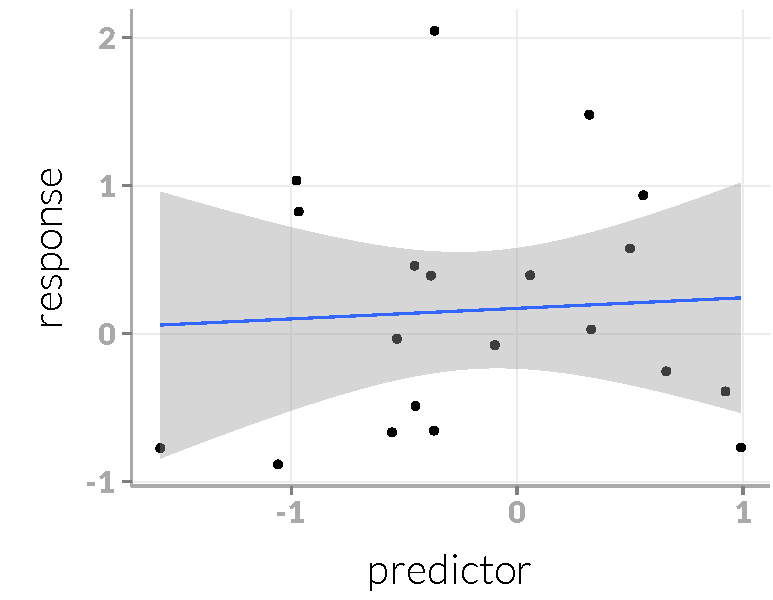
\includegraphics[width=0.8\textwidth]{figure/figPlots-1} 

}

\caption[A cruddy figure.]{
Caption labels can be really long so they might want to be separate. 
You can't have split lines in the knitr chunk options.
You figure legends should be version controlled too!
}\label{f:figPlots}
\end{figure}


\end{knitrout}

\section{Methods}

Remember to put results directly into text with \texttt{\\rinline}.
My model for this chapter isn't great (p = 0.8).







\small
\printbibliography 

\end{document}
